\documentclass[border=8pt]{standalone}
% shared preamble for lecture topic figures (compile from beamer/ with xelatex)
\usepackage{tikz}
\usepackage{fontspec}
\usepackage{amsmath}
\usetikzlibrary{arrows.meta,positioning,calc,backgrounds,fit,decorations.pathmorphing}
\setsansfont{SpaceGrotesk}[Path=fonts/,Extension=.ttf,UprightFont=*-400,BoldFont=*-700,FontFace={md}{n}{*-500}]
\renewcommand{\familydefault}{\sfdefault}
\definecolor{navy}{HTML}{182B49}
\definecolor{gold}{HTML}{C8881E}
\definecolor{teal}{HTML}{1F6F86}
\definecolor{green}{HTML}{157E6B}
\definecolor{stone}{HTML}{F7F6F2}
\definecolor{ink}{HTML}{182B49}
\tikzset{
  card/.style={fill=white, rounded corners=4pt, draw=navy!15, line width=0.5pt},
  flow/.style={-{Stealth[length=4pt]}, navy, line width=0.9pt},
  lab/.style={text=navy, font=\sffamily\fontsize{8}{9}\selectfont},
  toplab/.style={text=navy!65, font=\sffamily\fontsize{8.5}{10}\selectfont},
}

\begin{document}
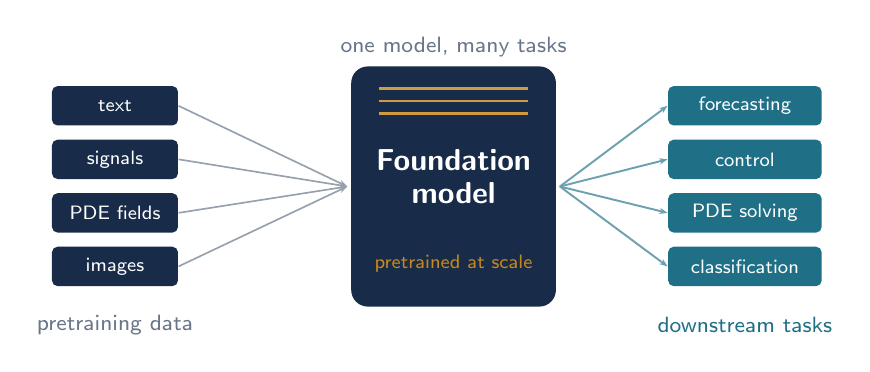
\begin{tikzpicture}
  \node[toplab] at (4.3,3.25) {one model, many tasks};
  % diverse pretraining data (left)
  \foreach \i/\lab in {0/text, 1/signals, 2/PDE fields, 3/images}{
    \node[fill=navy, text=white, rounded corners=2pt,
          font=\sffamily\fontsize{7.5}{9}\selectfont, minimum width=1.6cm, minimum height=0.5cm]
          (d\i) at (0,{2.5-\i*0.68}) {\lab};
  }
  \node[lab, text=navy!65] at (0,-0.28) {pretraining data};

  % big foundation-model block
  \fill[navy, rounded corners=6pt] (3.0,-0.05) rectangle (5.6,3.0);
  \foreach \i in {0,1,2}{\draw[gold!85, line width=0.9pt] (3.35,{2.4+\i*0.16}) -- (5.25,{2.4+\i*0.16});}
  \node[white, font=\sffamily\bfseries\fontsize{10.5}{12}\selectfont, align=center] at (4.3,1.6) {Foundation\\model};
  \node[gold, font=\sffamily\fontsize{7}{8}\selectfont] at (4.3,0.5) {pretrained at scale};

  \foreach \i in {0,1,2,3}{\draw[-{Stealth[length=3pt]}, navy!45, line width=0.6pt] (d\i.east) -- (2.95,1.475);}

  % downstream task heads (right)
  \foreach \i/\lab in {0/forecasting, 1/control, 2/PDE solving, 3/classification}{
    \node[fill=teal, text=white, rounded corners=2pt,
          font=\sffamily\fontsize{7.5}{9}\selectfont, minimum width=1.95cm, minimum height=0.5cm]
          (t\i) at (8.0,{2.5-\i*0.68}) {\lab};
    \draw[-{Stealth[length=3pt]}, teal!65, line width=0.7pt] (5.65,1.475) -- (t\i.west);
  }
  \node[lab, text=teal] at (8.0,-0.28) {downstream tasks};
\end{tikzpicture}
\end{document}
